% !TeX root = ../main.tex
% Add the above to each chapter to make compiling the PDF easier in some editors.

\chapter{Introduction}\label{chapter:introduction}
Cloud computing moves towards smaller deliverables. First hardware,then infrastructure, virtual machines, platforms, containers, and functions. While customers are facing with smaller deliverables, the background stays mostly the same. Even if the user only deploys a function, cloud provider creates an OS and deploys a containerized application that runs the given user function. There are at least 3 different abstractions between what user wants to run (their function) and what runs it ( hardware). That's 2 times more than the desired abstraction level. There should be other ways to decrease the distance between the hardware and the user application without compromising the flexibility of cloud computing. 
\begin{figure}[htpb]
  \centering
  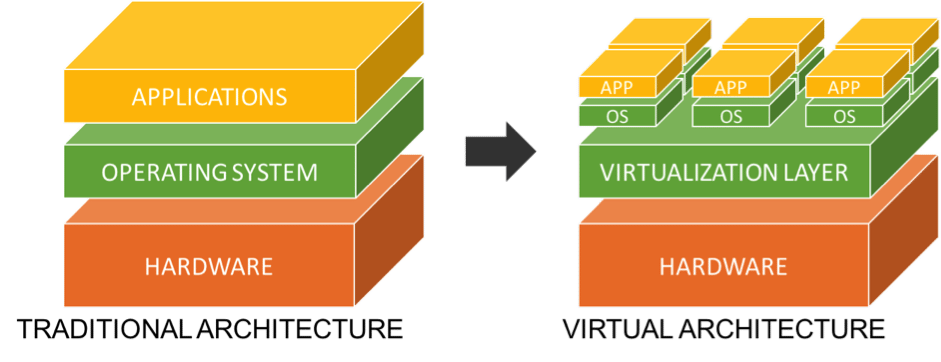
\includegraphics[width=0.8\textwidth]{figures/1-123.png}
  \caption{Moving from traditional architecture to virtualization based architecture: https://resources.infosecinstitute.com/11-points-consider-virtualizing-security/} \label{fig:arch}
\end{figure}
\section{Motivation}
Unikernels are special programs that package application code together with a minimal operating system image.\cite{7396164} These special programs can be booted like operating systems and more interestingly , they can also be virtualized like operating systems. That means we can do , in theory, any scheduling operation we normally do on virtual machines with unikernels. In the current world of orchestration technologies , this opens many new areas to apply the principles of deployment, scaling and scheduling.

Kubernetes is an open source system for automating orchestration of containerized applications. \cite{Hightower:2017:KUR:3175917} Kubernetes by default uses Docker as it's runtime. Both it's own services and user defined services are deployed as docker containers. Instead of communicating with virtual machines running on the Kubernetes cluster, user only interacts with the Kubernetes API and it schedules deployments according to rules. 

The docker runtime requires a host operating system to run the docker daemon, thus this requires every node to have a full fledged operating system to run even simple applications. Those operating systems also run background jobs that come with the OS but not required by the running applications. E.g. a usb driver or a sound driver is not vital for a web application but operating system still runs them by default. Unikernel programs package only functions required by the running application in a different configuration. That decreases the scaling time\cite{Podolskiy:2017:QCA:3069383.3069390} of the applications because first no operating system is required to boot up, and second the applications are much more smaller , so they can be downloaded faster.

The proposed effects of a kubernetes cluster running together with a unikernel system can be summarised as follows: 

\subsection{Security}
 These OS's are required for the multi-tenant cloud architecture for isolation. Otherwise, vulnerability in one of the containers can compromise all other containers running on the same VM. On the other hand, a vulnerability found in the operating system can also compromise the running applications. Unikernels packages only include required parts of the operating system so the attack surface is greatly reduced.

\subsection{Resource Utilization}
The user never interacts with the underlying operating system that their application is running on. It is only used by cloud provider infrastructure. Nevertheless, the user still pays for the resources used by the operating system, even though their application doesn't. 

\subsection{Scaling Time}
Unikernels have a very small footprint and can run on hardwares only with a hypervisor.

\subsection{IoT Scenarios}
Unikernels also have role in the IoT world. Their size allows them to be deployed to places with sparse internet connection or low-end devices. Their security story makes them hard targets in the IoT ecosystem, where security practices are still a challenge for developers. \cite{iot-sec} On the other end, the single-address space feature of unikernels is a downside for their usage in IoT applications, because it makes it hard for unikernels to read sensor data from the device itself. Nevertheless, for simple, proof of concept applications, kubernetes can be used to schedule them to IoT devices. Kubernetes comes in handy for such scenarios, because users can tag deployments they make and K8s will deploy them to their respective devices. Multiple unikernel applications can be deployed to the same device with a single deployment through the Kubernetes API or resources provided by the IoT devices can be accessible from the Kubernetes , and unikernels can be deployed to those. Given that multiple unikernels can run on the same device, a microservice based architecture can also be used for IoT programs where a single unikernel is tasked with only one job and it communicates with other unikernels through a shared medium locally on the device or through Kubernetes services. This brings the advantages of microservice based development to the IoT domain.


\section{Research Problem}
\subsection{Deployment}
Unikernels can be booted only in systems that either have a type-1 or a type-2 hypervisor. While they can be booted directly from BIOS on hardware, this does not give the flexibility required by cloud computing standarts so a hypervisor is required to boot up and remove programs to achieve the desired state by the system.

Type-2 hypervisors run on a host operating system and they are easier to work with. If they provide an API, the host operating system can be used to develop programs to communicate with them. Given an example , a linux machine with virtualbox installed can boot up unikernel programs with terminal commands and no GUI is required. Then ,this terminal commands can be automated with a program that communicates with the internet.

For type-1 hypervisors, the task at hand is harder. There is no operating system involved and one has to work mostly with the API provided by the hypervisor itself. This calls for a program that either can be deployed to the hypervisor as a unikernel itself or for a virtual machine that can talk with the underlying hypervisor.


\begin{figure}[htpb]
  \centering
  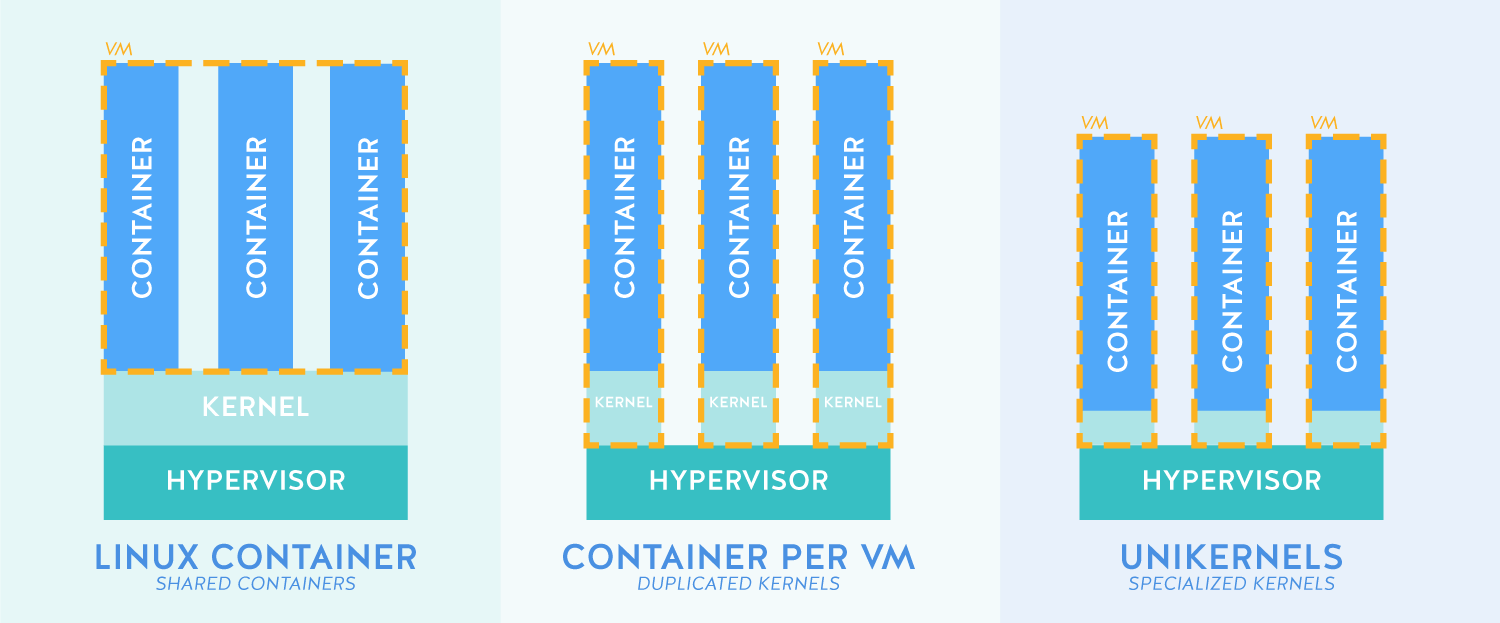
\includegraphics[width=0.8\textwidth]{figures/Linux-containers-vms-unikernels.png}
  \caption{Different virtualization techniques: https://nordicapis.com/introduction-to-unikernels/} \label{fig:virt}
\end{figure}



\subsection{Virtual Kubelet}
Virtual Kubelet\cite{virtual} is a Microsoft project that aims to provide a programmable kubelet API interface for developers. It allows to deploy Kubernetes resource to different runtimes, transparent to the Kubernetes API. This project is currently a great candidate to deploy the unikernel solution proposed by this thesis. Virtual kubelet communicates with a custom pods provider to deploy resources. If the implementation of this thesis follows this approach, Virtual Kubelet will be forked and a new provider will be written for certain hypervisors to deploy unikernels. This also gives the opportunity to do a pull request to the project directly at the end of this thesis.

\begin{figure}[htpb]
  \centering
  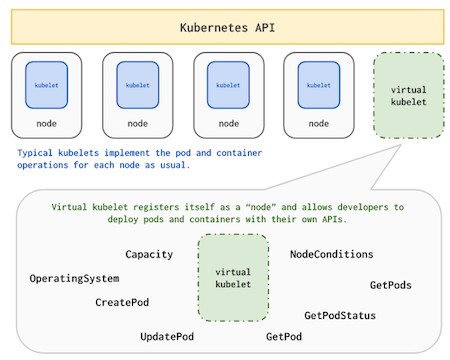
\includegraphics[width=0.8\textwidth]{figures/vk.png}
  \caption{Working principle of Virtual Kubelet \cite{virtual}} \label{fig:vk}
\end{figure}

Virtual Kubelet also opens possibilities to deploy unikernels to IoT devices through the Kubernetes API. Different virtual kubelet instances with different providers can work in parallel to deploy to target environments. This, again requires a receiver on the IoT device part. 
\subsection{Kubernetes service discovery}
Kubernetes has a built-in service discovery. Deployed containers use hostnames instead of IPs to communicate between each other. Kubernetes runs a DNS server and maps those hostnames to IP addreses of individuals containers or mostly services. Unikernel deployments should also have the same functionality to work flawlessly with the rest of the kubernetes cluster. 

\subsection{Communication between kubernetes and hypervisor}
Kubernetes has a single endpoint for all the communication between the user and the cluster. This single endpoint should be aware of unikernel deployments so that it can schedule them accordingly. Kubernetes provides different ways to achieve this extensibility. First, it allows developers to create custom resource definitions such that they can be used together with other kubernetes resources. Second, kubernetes allow for deployment for different scheduler that can operate on specificly-tagged deployments. 

\section{Proposed Solution}

Before starting to implement unikernels to Kubernetes, a couple of proof of concept unikernel programs will be created. To create those programs, open-sourced unikernel solutions will be used. There are multiple projects with different approaches and different runtime environments. Next chapter explains more about those solutions. Selecting the most suitable one for the purpose of this thesis plays a crucial role because, it is out of scope for this thesis to develop a new unikernel solution just for Kubernetes. Once those programs are created, unikernel deployments will be added to kubernetes arsenal with the following steps:

1) A node with a type-2 hypervisor will be created. A custom program will be written that takes orders from a server and boot up unikernels according to parameters coming from the order. The custom program will run on the host operating system and there will be no kubernetes involvement.

2) A kubernetes cluster will be created and that custom program will be modified to communicate with kubernetes. Everytime a unikernel deployment is made, kubernetes will notify this program, and program will do the deployment.

3) Kubernetes DNS system will be integrated to the node with the type-2 hypervisor so they can communicate with other applications.

4) A node with a host operating system with type-1 hypervisor will be created. E.g. Xen hypervisor can also run on a host operating system. This node will be modified to communicate with the kubernetes cluster through the host operating system. 

5) A node without a host operating system with type-1 hypervisor will be created. This node should also run the custom program that communicates with the kubernetes cluster on the hypervisor and should also do the networking of unikernels between other kubernetes resources.This will be the final outcome of the thesis.

\begin{figure}[htpb]
  \centering
  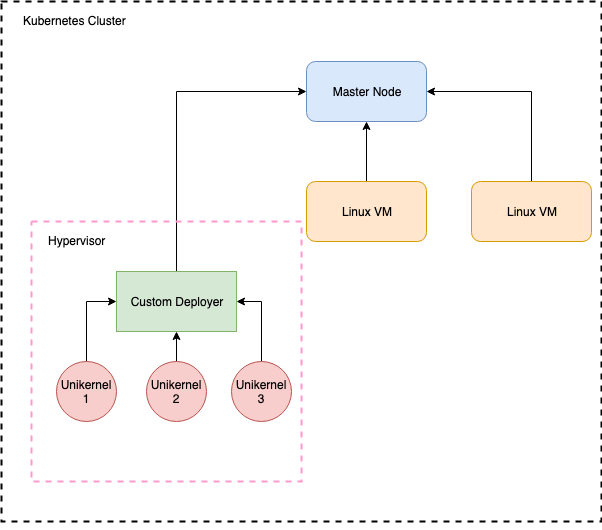
\includegraphics[width=0.8\textwidth]{figures/arch3.png}
  \caption{A kubernetes cluster with a only hypervisor enabled node for unikernel deployment} \label{fig:hypervisor}
\end{figure}


A scope of this project is not to come up with a new unikernel solution and it will use the ones already developed by the open-source community.It also won't compare application performance between docker containers and unikernels. It will although compare the deployment time between those.
